\documentclass[]{article}
\usepackage[left=3cm,right=3cm,top=1.5cm,bottom=2cm,includeheadfoot]{geometry} 
\usepackage{babel}
\usepackage{hyperref}
\usepackage{mwe}
\usepackage[markcase=noupper]{scrlayer-scrpage}
\usepackage{amsmath}
\usepackage{amssymb}
\usepackage{multirow}
\usepackage{subcaption}
\usepackage{rotating}

% bibliography natbib
\usepackage{natbib}
\bibliographystyle{abbrvnat}
%\setcitestyle{authoryear, open={((},close={))}
\renewcommand{\cite}{\citep}


% configure headline

\ihead{Tilman Hinnerichs}
\ohead{Linking Connectivities and Gene Expression Patterns in the Mouse Brain}
\cfoot*{\pagemark}
%opening
\title{Linking Connectivities and Gene Expression Patterns in the Mouse Brain}
\author{Tilman Hinnerichs}
\date{}
\pagestyle{headings}

% Build subsubsubsection
\usepackage{titlesec}
\usepackage{todonotes}

%Definitions
\newtheorem{mydef}{Definition}
\newtheorem{example}{Example}
\newtheorem{lemma}{Lemma}
\newtheorem{theorem}{Theorem}
\newtheorem{corollary}{Corollary}
\newtheorem{proposition}{Proposition}

\newcommand{\name}{Treasure}

\newcommand{\HRule}[1]{\rule{\linewidth}{#1}}
\setcounter{tocdepth}{5}
\setcounter{secnumdepth}{5}

%-------------------------------------------------------------------------------
% TITLE PAGE
%-------------------------------------------------------------------------------

\begin{document}
	
\pagenumbering{gobble}
	
\title{ \normalsize \textsc{Diploma thesis}
	\\ [2.0cm]
	\HRule{0.5pt} \\
	\LARGE \textbf{\uppercase{Linking Connectivities and Gene Expression Patterns in the Mouse Brain}
		\HRule{1pt} \\ [0.5cm]
		\normalsize September 30, 2022 \vspace*{5\baselineskip}}
	
	\date{Summer semester 2022}
	
	\author{
		Tilman Hinnerichs \\
		Matrikelnummer: 4643427 \\ 
		Technische Universität Dresden\vspace{1cm}\\
		Tutor: Dr. Nico Scherf\\
		MPI for CBS}}
\maketitle
\todo{proper title?}
\newpage
\begin{abstract}
	
\end{abstract}

\newpage

\tableofcontents

\newpage


\subsection*{To be sorted somewhere}
\begin{itemize}
	\item Variability and different interpretations of different graph convolutional neural filters \cite{GCNConv, GENConv2020, feng2022kergnns} etc.
	
	
	\item DeepGOPlus for feature generation \cite{DeepGoPlus}
	\item discussion of different PPI network databases \cite{STRINGv10}
	\item discussion of potential databases associating gene expression data with their spatial distribution \cite{hawrylycz_digital_2011}
	\item discussion of best neural learning/graph convolutional methods \cite{Pytorch, PytorchGeometric}
	\item how to handle highly imbalanced data, metrics, preprocessing, sampling, modification of loss function \cite{Jeni2013} and optimization over them (with Adam\cite{Adam2014})
	\item maybe introduction of PhenomeNET for MP/GO for more sophisticated protein representation \cite{PhenomeNET2011, GOoriginal2000, GOrecent2020, MP2009} and derive features from DL2vec \cite{DL2vec2020, Word2vec2013}
	\item evaluation of \glqq Using ontology embeddings for structural inductive bias in gene expression data analysis\grqq{}\cite{Trebacz2020}
	\item take some ideas from \citet{Zitnik2017} with title \glqq Predicting multicellular function through multi-layer tissue networks\grqq{}. (OhmNet)
	\item potentially group results based on InterPro\cite{Interpro2020} families eventually
	
	\item choice of model organism?!
\end{itemize}


\newpage
\pagenumbering{arabic}

\section{Introduction}
\label{sec:introduction}
General thread for introduction and motivation:
\begin{itemize}
	\item Gene expression patterns are difficult to analyze in humans $\rightarrow$ take mouse as model organisms
	\item why do we study sane mice and not a
	
	\item The brain is a multi-level system in which the high-level functions are generated by low-level genetic mechanisms. Thus, elucidating the relationship among multiple brain levels via correlative and predictive analytics is an important area in brain research. Currently, studies in multiple species have indicated that the spatiotemporal gene expression patterns are predictive of brain wiring. Specifically, results on the worm Caenorhabditis elegans have shown that the prediction of neuronal connectivity using gene expression signatures yielded statistically significant results.
	\item no in-depth analysis of mouse brain genetic patterns and their relation to different connectivity patterns has been made yet

	\item Why are we concerned with gene expression prediction and what could it tell us?
	\begin{itemize}
		\item \cite{twine2011whole} show the importance of gene expression patterns, by linking gene expression abberation with increase in Alzheimer's disease
		\item studies have shown circadian patterns of gene expression in human brain and the disruption of those in depressive disorder \cite{li2013circadian}
		\item first understand sane brain and its circuits, before tackling pathological data
	\end{itemize}
	\item why is finding (low-dimensional) patterns important here?

	\item What is structural and functional connectivity and what are associated hypotheses? 
	\begin{itemize}
		\item \cite{fornito2015connectomics} elaborate on the connectomics of brain disorders and its complexity in connectivity. Understanding how brain networks respond to pathological perturbations is crucial for understanding brain disorders and behavior
	\end{itemize}
	\item Why is finding a link or to connectivity from gene expression desirable?


	\item Why do we think that GCNs could help finding such patterns?
	\begin{itemize}
		\item Guilt by association over gene networks \cite{Oliver2000, Gillis2012} in genetic networks
		
		\item protein function prediction from PPI networks \cite{Vazquez2003}
		\item GCNs have been applied successfully to variety of tasks over different types of graphs.		
	\end{itemize}

	\item what are our contributions?
	\begin{itemize}
		\item Showed that graph convolution over PPI graphs helps finding patterns in gene expression data
		\item Contributed an implementation of our method
		\item contributed an implementation of KerGNN to PyTorch Geometric
		\item built an open framework for parametric UMAP in torch to integrate non-UMAP graphs
	\end{itemize}
	\item what is the outline of this script?
	\item implementation available at Github link
\end{itemize}

\subsection*{General Introduction of the Research Study}

\subsection*{Research problem or Questions with Sub-Questions}

\subsection*{Reasons or Needs for the Research Study/Motivation for my research}

\subsection*{Definition and explanation of Key Terminology}

\subsection*{Context of Research Study within th Greater Discipline}

\begin{itemize}
	\item Introduction to mouse brains as model organisms for insights into human brain
	\item Works on mouse brain in general and potential tasks
	\item works on gene expression in mouse brains
	\begin{itemize}
		\item traditional approaches
		\item importance of gene expression patterns in mouse brains
	\end{itemize}
	\item neural networks for this purpose
	\begin{itemize}
		\item how were 
	\end{itemize}
	\item gene expression for general tissue
	
\end{itemize}

\newpage
\section{Literature overview}
\label{sec:relatedwork}
\subsection{Gene expression databases and prediction}
\label{sec:relatedwork_geneexp}
Research in gene expression prediction and profiling has a long history in bioinformatics and systems biology, but was almost exclusively linked to cancer research. Moreover, with the rise of machine learning, and more specifically (deep) neural networks and its variants, this field became increasingly data reliant. The Human Genome Project \cite{watson1990human}, launched in 1990 and declared finished in 2003 while the first gapless assembly was finished in 2022, also sparked various works in relating these genetic representations to other tissue- and individual-specific properties and traits.\\ 

For comparison of gene expression profiling works there exist multiple prominent variables. Most significantly, the chosen organism is a crucial choice for both data availability and predictive complexity. Second, the chosen tissue is naturally important for the proposed hypotheses, especially with respect to tissue definitive cancer research, and its potential ability to generalize without transfer learning. While gene expression pattern analysis approaches frequently focus on tissues like \textit{mamma}, (primarily female) breast, \cite{herschkowitz2007identification}, liver \cite{flores2002patterns}, and skeletal muscle \cite{lecker2004multiple} for exploration of diseases like cancer and atrophy, respectively, in humans. 

However, the nervous system is often investigated separately as it bears different molecular processes and structure, anatomy and cell life cycles, while brain and spinal cord are even based in a separate nutritional circuit for mammals. Moreover, gene expression determination in the human brain may almost certainly remain an deadly intervention for most brain tissues, hence allowing only for careful extraction of specific tissues in living organisms. Also this disallows for \textit{in-vivo} extraction of vital brain regions and structures, e.g. the brainstem. Furthermore, the human brain's gene expression patterns are varied and diversified \cite{ramasamy2014genetic}, aligning with its anatomical and embryogenesis complexity, and its compartments are exceptionally and deeply connective and collaborative \cite{fornito2015connectomics}. Both also hold for invertebrates, i.e. insects. Thus, full genetic profiles of expression are mandatory for a full understanding of the mammalian and invertebrate brain and primary nervous system, respectively. By the strong intervention of the tissue extraction, full genome atlases are fit together from various experiments on multiple individuals.

The human brain is among the most intricate and complicated networks we do know of, and is far from being fully understood. Additionally, full transcriptomic atlases of human brains are difficult to collect while raising decisive privacy concerns. Yet, there were multiple efforts and projects with rather small sample sizes. A detailed elaboration on dataset and organism choice, and their respective properties may be found in Section \ref{sec:datasets}. \\

However, there have been works on numerous works for other tissues and other organisms. \citet{modencode2010identification} correlate activity patterns in the regulatory network within \textit{Drosophile}, proposing their model for identification of functional elements "modENCODE". As this work was published back in \citeyear{modencode2010identification}, the approach relies purely on statistical correlation and covariance. \citet{chikina2009global} follow a similar approach in \textit{C. elegans} predicting tissue-specific gene expression in \citeyear{noble2006support} utilizing support-vector machines (SVM)\cite{noble2006support}. 

More modern, data-oriented machine learning models such as (deep) neural networks (NN) were applied successfully to similar problems. \citet{aromolaran2020essential} achieved to predict essential genes based on their respective sequence and functional features profiting off NNs, while transcriptomic interaction prediction was done based on functional gene data using deep learning in \citet{yang2019predicting} in \textit{Drosophila} over different tissues. 

Within humans, as mentioned previously, gene expression was primarily used for cancer and disease research. \citet{schulte2021integration} and \citet{wang2021mogonet} were the first to apply graph convolutional neural networks to the task of gene expression prediction within humans. While \citet{schulte2021integration} was applied on data from The Cancer Genome Atlas (TCGA)\cite{tomczak2015review} across multiple tissues, \citet{wang2021mogonet}'s MOGONET is proposed as a general framework for gene expression prediction with example computations on ROSMAP dataset and TCGA. Both approaches implement the original formulation of GCNs\cite{GCNConv}, which we will discuss in more detail in Section \ref{sec:graphconv}, over protein-protein interaction networks and accomplish outstanding performances and both measure biomarker importance for prediction in order to leverage explainability. The authors thereby exploit the "guilt by association" principle \cite{Oliver2000, Gillis2012} over gene networks, adding background knowledge such as biological interaction and pathways.

Crucial for almost all classification tasks in machine learning is the choice of entity representation. In the mentioned works molecular \cite{schulte2021integration, modencode2010identification, noble2006support} and phenotypical \cite{wang2021mogonet, chikina2009global} features were used for expression prediction, but never both combined. The combination of phenotypical and molecular features over GCNs was proven to raise predictive performance in drug-target interaction prediction \cite{hinnerichs2021dti} but remains an open challenge for this very task.


\subsection{Finding spatial patterns in gene expression in mice brains}
\label{sec:relatedwork_micebrains}
In this subsection we will constrain the issue of gene expression analysis to both "spatial patterns", mammals and the tissues of the brain, which we study in this work. The term \textit{spatial patterns} is rather vague and allows for various interpretations, both discrete and continuous, which will form the classes for the following literature review.\\

In \citet{pavlidis_analysis_2001} is the first first review paper on regional variation in genetic expression in mouse brain, up to our knowledge.  
\citet{zapala2005adult} is also among the earliest works, showing that local structures beared "transcriptional imprint" that coincide with the embryological origin of the examined regions. However, they only were able to identify up to 24 neural tissues. They further conclude that this may be important for functional collaboration within the adult mouse brain. The authors measure pairwise correlation show the existence of clusters over a heatmap. \\

The Allen Institute Brain Atlas (AIBA), is a collection various atlases such as Allen Mouse Brain Atlas (AMBA)\cite{MouseBrainAtlas, daigle2018suite}, the Allen Mouse Brain Connectivity Atlas (AMBCA) \cite{oh2014mesoscale, harris2019hierarchical} and the Allen Mouse Brain Common Coordinate Framework (CCFv3) \cite{wang2020allen} to name only the ones related to adult mice's brains. As it was the first coherent collection of spatially resolved expression values, mapping 2D expression images consistently to 3D coordinates, the AMBA has sparked a range of publications. Within \citet{MouseBrainAtlas}, the Allen Institute also published the "Allen Reference Atlas"(ARA) proposing a number morphological and histologically induced sub-regions of the brain and hence a precisely defined parcelation. Moreover, they propose the ARA \textit{ontology}, a semnatic hierarchy, providing a hierarchical cluster of all sub-structures and map them back to their coordinates with the CCF. 

\todo{Name a few "sparked"  research works on this}

\citet{bohland2010clustering} advance clustering of such expressions under usage of singular value decomposition (SVD) within mice, combined with an extensive analysis of similarities to neuroanatomy.
Likewise, \citet{takata_flexible_2021} propose a flexible annotation atlas of the mouse brain, introducing a flexible ontology construction framework which may be used on the transcriptomic data such as the AMBA, leveraging anatomic structure and axonal projection data. Here, FAA focuses on consistent and reproducible regions-of-interest (ROIs) definition for other downstream tasks such as resting-state functional connectivity annotation. Further, this ontology may be seen as a pattern within mouse brain, while it may only detect connected structures. 

The authors of \citet{ValkShapingBrainStructure2020} analyze structural covariance of cortical thickness within primate brains, namely macaques, and its correlation to each cortical layers transcriptome. Further, transcriptomic variation was related to a continuum of functions by mapping them the brain anatomy, inducing a \textit{continuous}, functional parcelation of the primates brain. Further, this study suggests a relation of functional and transcriptomic links. Similarly, \citet{zeng_deep_2015} propose a range of deep learning methods for capturing spatiality of gene expression within the mouse brain. A notable addition is the work of \citet{kelly_graphsim_2020}, presenting an R package for simulating gene expression from graph structures over general biological pathways, that may be and was applied to (mammalian) brains prospectively. 

While also focused on mouse brains, \citet{Partel2020} submits a novel database based on their own \textit{in-situ} sequencing data, and a consecutive spatial gene expression analysis pipeline, and relates the results to tissue morphology and hence indirectly to the AMBA. Similarly to our proposed approach, brain parcelation are present as $n$-dimensional, continuous embeddings, representing closeness in gene expression space.  Due to the similarity in the pipeline especially in their visualization utilizing UMAP, we will use the generated images of this work for a brief comparison in Section \ref{sec:results}.

Up until now, GCNs were not applied to this issue.

\subsection{Structural and functional connectivity prediction}

In this section we will examine related work on brain connectivity prediction from transcriptomic data. We hereby separate axonal and functional connectivity due to their differing associated hypotheses.\\

The relation of gene expression patterns and \textit{structural} connectivity was studied numerous times over various model organisms, especially\textit{C. elegans}, \textit{Mus musculus}, but also humans. We will categorize existing literature with respect to the underlying organism.

\citet{kaufman2006gene} and \citet{varadan2006computational} were among the earlier works on this research field, followed by \citet{arnatkevic̆iute2018hub}, showing the relation of axonal connectivity and gene expression within \textit{C. elegans}. 
Further, that relation was shown by \citet{rubinov2015wiring}, \citet{fakhry2015global} and \citet{fulcher2016transcriptional} for the mouse brain, while \citet{parkes2017transcriptional} and \citet{goel2014spatial} proved a correlation within human brains.

\citet{fakhry2015high} is among the earlier works focusing on the predictive power across different mouse brain regions. They applied non-machine learning, computational models for axonal connectivity prediction in adult mouse brains. Similarly, \citet{roberti2019exploiting} uses transcriptomic information to anatomical connectivity patterns and gene expression of neurons using (shallow) neural networks. Yield a 85\% accuracy in prediction of unconnected and connected regions. Both shall serve as a baseline performance in chapter \ref{sec:results}. 
Only recently, \citet{wang2022network} proposed a novel-network based method integrating molecular-based gene association networks such as protein-protein interaction networks with brain connectome data. They further link these gene expression patterns to four brain diseases, including Alzheimer’s disease, Parkinson’s disease, major depressive disorder and autism.
\\

The correlation of \textit{functional} connectivities and transcriptomic data is much more complex in nature than the previous task. We will again classify approaches by their respective model organism.

\citet{whitfield2003gene} were one of the first to link transcriptomic data with behavior and hence functional patterns in individual honey bees back in \citeyear{whitfield2003gene}. The authors show that changes in the messenger RNA were connected to behavior and how changes to RNA directly influenced the other.
\citet{rankin2002gene} first developed the idea of combining behavioral analyses of \textit{C. elegans} with their genetics. Further, \citet{sun2021temporal} only recently described the distinct functional states and the corresponding distinct molecular states within the transcriptome. While honey bees and nematodes are rather simple model organisms, enabling both full transcriptomic analyses of the organisms, and their bearing and actions. However, "behavior" may be ambiguous and vague for such taxonomically distant animals, from the viewpoint of humans, and may only be linked to very basic meta-tasks such as basic routing, orientation and basic social interaction. 

Research on humans further indicates correlation of transcriptomic patterns and "neural dynamics", concluded from e.g. fMRI data \cite{richiardi2015correlated, diez2018neurogenetic, vertes2016gene} or electrocorticography \cite{betzel2019structural}. We refer to \citet{fulcher2021overcoming} for an extensive overview on the link to axonal and functional connectivity. Further, \citet{Zerbi2021} propose a computational model calibrated over 16 autistic mouse models, that reveals a range of functional connectivity subclasses and -types.


\subsection*{Brief Overview of LIterature Reviewed, Discussed and applied}

\subsection*{Study Model and Process Aligning with literature reviewed}

\subsection*{Hypotheses and justifications tied to prior sections and statements}

\subsection*{The Scope of the study with theoretical assumptions and limitations}


\newpage
\section{Materials and methods}
\label{sec:methods}
In this study, we utilized and incorporated various approaches from other works and applied them to diverse datasets. The following section will give a brief overview over all modules of the proposed models, while the entire computational methods will be presented and described in the results section (Section \ref{sec:results}). We further introduce the goals and scopes of our respective research questions and on our evaluation metrics for this purpose.  
\subsection*{Introduction and general description, study method and study design}
\subsection{Problem description}
\label{sec:probdesc}
Here we give a brief introduction to each of the three tackled issues and further summarize data properties, challenges and goals of each problem in this section and Section \ref{sec:datasets}. 
\subsubsection{Spatial gene expression prediction}
\label{sec:probdesc_geneexp}
Firstly, the issue of spatial gene expression prediction is concerned with the following problem: Within a given structure or at a specific coordinate, and for a given gene, we want to determine whether the latter is expressed or not. While there are also ways to quantify the expression within a region, we only care about the \textit{quality}, i.e. whether the is expressed or not. We treat all structure-gene pairs without a known expression as negatives, thus handling the dataset in a closed-world manner, and accordingly formulate the problem as a binary classification task. Naturally, as shown in Section \ref{sec:relatedwork_micebrains}, mammalian brains show a high correlation of gene expression and neuroanatomic substructures, suggesting importance of nearby and adjacent structures to the considered one. While spatial prediction and conditionals are hard to infuse into models, we will therefore start by predicting gene expression within single structures, constructing train and validation set over genes, or train from related or proximate regions.

\subsubsection{Preserving dimensionality reduction in brains}
\label{sec:probdesc_dimpres}
The second studied issue is the task of preserving dimensionality reduction. Here, all regions or 3D-voxels are associated with a vector embedding of fixed dimensionality $n$, representing each section with the features of choice. As we are concerned with the influence and patterns of gene expression we will only use and consider embeddings of transcriptome for this task. The eventual task is to find a mapping $f_{emb}:\mathbb{R}^n \rightarrow \mathbb{R}^k$ with $k<n$ reducing each structure's representation dimensionality to $k$, such that the relative, pairwise distances are preserved. Hence, if two sections share similar expressions, they should be described similarly in $\mathbb{R}^k$, invariant to spatial distance. As we seek to visualize such embeddings for quality assessment of the embeddings and characterization of marked regions, a mapping into color-space, i.e. choosing $k\in\{1,2,3\}$, appears natural.

\subsubsection{Structural and functional connectivity prediction}
\label{sec:probdesc_connpred}
Eventually, we want to forecast the brain's connectome in our third formulation: Given two structures we want to predict whether there is a connection either of axonal or functional or both types. Therefore, similarly to the question of dimensionality, regions and voxels, respectively, are represented by their expression characteristics in vector space. Likewise to other works, introduced and explained in Section \ref{sec:results}, and to the issue described in \ref{sec:probdesc_geneexp}, our analysis is invariant to the eventual "strength" of the connection, but focuses on the quality of connectivity. Hence, we define a cut-off threshold converting the issue to a binary classification task, whereas non-positive and unknown links are treated as negatives.


\subsection*{Assumptions of study method and study design with implied }

\subsection{Datasets and preprocessing}
\label{sec:datasets}
As human brains are among the most complex in structure and connectivity within nature, a full transcriptomic atlas may be very valuable for the research community and our experiments in this work. However, full transcriptomic atlases of homo sapiens are ethically difficult to gather. Additionally, as a valuable, public genetic atlas of deceased relatives may provide highly critical information about the remaining, living ones, such as genetic diseases, genetic markers for correlating with addiction and other social behavior, or ancestry in general, this raises tremendous privacy concerns. As we aim to investigate transcriptomic patterns in the brain and their relation to structural and functional connectivity as a generalized, organism-invariant methodology, we also want our experiments to be as understandable and replicable as possible. 
However, there have been multiple initiatives towards collaborative and open human brain data, such as the Allen Human Brain Atlas (AHBA) \cite{hawrylycz_digital_2011} also published by the Allen Institute and the Human Brain Atlas (HBA) \cite{roland1994human}. While both are almost complete, e.g. AHBA considers over $20000$ genes, but these were collected from just 6 human individuals. In combination with the Human Connectome Project (HCP) \cite{van2013wu} this atlas provides a valuable, matched data resource. As rodents, and more specifically mice, are more simplistic and well studied in behavior and due to their taxonomic proximity to humans serve as model organisms for diverse genetic, social and medical experiments, we opted for mice as the study organism. The ultimate goal still shall be the further understanding of brains of our species.

Furthermore, immense effort was put into enormous projects and databases for model invertebrates, namely \textit{Drosophila} (specifically \textit{Drosophila melanogaster}, also called \textit{fruit fly}) and \textit{Caenorhabditis elegans} (short: \textit{"C. elegans"}, colloquially also called \textit{roundworm}) with the two projects "Virtual Fly Brain" \cite{milyaev2012virtual} (\href{https://virtualflybrain.org/}{https://virtualflybrain.org/}) and "Wormbase" \cite{lee2003building, davis2022wormbase} (\href{https://wormbase.org}{https://wormbase.org}), respectively. Yet, we wanted to stay within the same taxonomic phylum leading our choice towards mouse brains.\\

We further use four different graphs in our setup, which shall be described and our choice motivated in the following sections:
\begin{enumerate}
	\item Structure -- gene expression data and the corresponding structure ontology/hierarchy, 
	\item Protein-protein interaction graph,
	\item Structural connectivity and axonal projection data, and
	\item Functional connectivity data.
\end{enumerate}

Links to all datasets and download scripts are available in the Github repository.

\subsubsection{Spatial gene expression values in mice brain}

The AMBA\cite{MouseBrainAtlas} is a genome-wise and comprehensive, digital 3D-map of spatial gene expression of the adult mouse central nervous system (CNS). AMBA utilizes \textit{in situ} hybridization (ISH) for expression measurement and is publicly and freely available. 
In literature there are several approaches, compromising sequencing depth, accuracy, throughput and spatial resolution. Generally, one can identify two classes of gene expression measurement while preserving spatial information. The first approach is to store spacial coordinates first, followed by a the sequencing of single-cell RNA where \citet{achim2015high} and \citet{chen2017spatial} propose the mapping and the Geo-seq protocol for this method. The second method includes the usage of "barcodes", decoded in the tissue sample, while running a parallel analysis of numerous mRNAs \cite{ke2013situ, moffitt2016high}. Here, AMBA and \citet{Partel2020}'s dataset are constructed using the first and the latter method, respectively. Sample extraction is very invasive and hence samples are collected from multiple individuals. Please see \citet{ng2007neuroinformatics} for more information and an overview on applied 3D reconstruction and registration of ISH images.\\

In AMBA over $17000$ genes were measured in voxels in resolutions of $10\mu m$, $25\mu m$, $50\mu m$ or $100\mu m$. An "average brain", i.e. averaging expression intensities of each voxel among all genes, is shown in Figure \ref{fig:average_cor} and \ref{fig:average_sag} as coronal and sagittal cross-sections.
The most important supportive dataset for AMBA is the Common Coordinate Framework Version 3 (CCFv3)\cite{wang2020allen} structuring  and mapping all brain voxels into identifiable sub-structures, based on their morphology. Unfortunately, functional connectivity (FC) measurement is often measured with respect to regions-of-interest (ROIs) that may coincide with these structures. Therefore, full brain FC datasets on voxel level may not be publicly available in the same resolution. Hence, for a full integration of all datasets, we will use the CCFv3 grouped voxel for structures, thus redefining all three problem descriptions from voxel to structure level, i.e. a set of voxels. A visualization of these structures based on the CCFv3 annotation volume is depicted in Figure \ref{fig:ano_cor} and \ref{fig:ano_sag}.\\


\begin{figure}
	\begin{subfigure}{.43\textwidth}
		\centering
		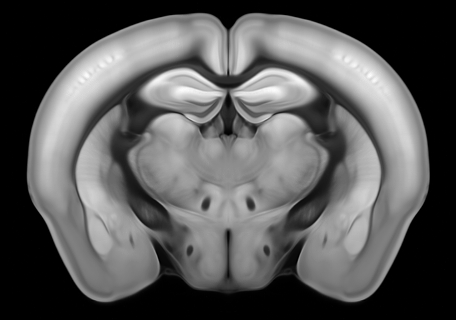
\includegraphics[width=.9\linewidth]{figures/avgt_coronal.png}
		\caption{Average coronal}
		\label{fig:average_cor}
	\end{subfigure}
	\begin{subfigure}{.3\textwidth}
		\centering
		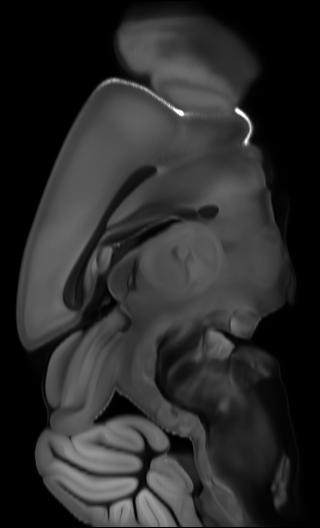
\includegraphics[width=.9\linewidth, angle=270]{figures/avgt_sagittal.png}
		\caption{Average sagittal}
		\label{fig:average_sag}
	\end{subfigure}\\
	\begin{subfigure}{.43\textwidth}
		\centering
		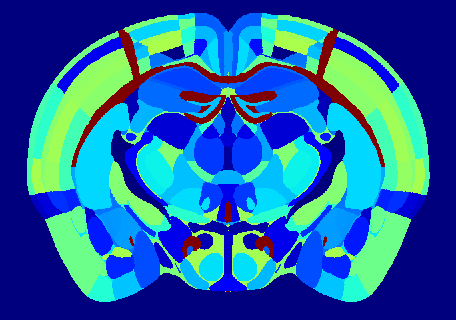
\includegraphics[width=.9\linewidth]{figures/ano_coronal.png}
		\caption{Annotation coronal}
		\label{fig:ano_cor}
	\end{subfigure}	
	\begin{subfigure}{.3\textwidth}
		\centering
		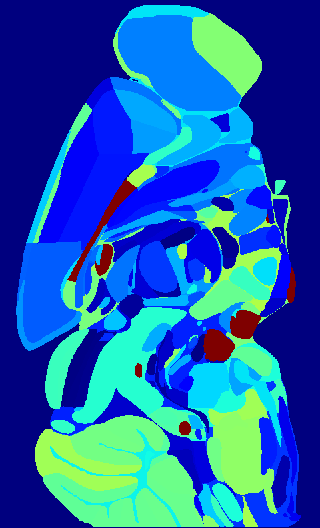
\includegraphics[width=.9\linewidth, angle=270]{figures/ano_sagittal.png}
		\caption{Annotation sagittal}
		\label{fig:ano_sag}
	\end{subfigure}
	\caption{(a)-(b): Coronal and sagittal view on the "average brain", an averaged map of all gene expression values gathered from AMBA; (c)-(d): Coronal and sagittal view on the annotation atlas, partitioning the reference brain into $\approx900$ sub-structures.}
	\label{fig:CCF_images}
\end{figure}

Expression values in AMBA are provided per structure as expression densities, intensities and energies. Let $g$ be the considered gene, $d$ the considered division or substructure, $P_{g,d}$ be the set of pixels within an ISH image and $P_{g,d,e}$ the set of expressing pixels, displaying expression of $g$ in $d$. Both $P_{g,d}$ and $P_{g,d,e}$ are given as measured expression intensities for the respective pixels. Thus, the three measurements are defined as shown in Table \ref{tab:expr_values}.

\begin{table}
	\renewcommand{\arraystretch}{3}
	\begin{tabular}{llp{8cm}}
		Metric name&Formula&Description\\
		\hline
		Expression density&$E_d:=\frac{|P_{g,d,e}|}{|P_{g,d}|}$&sum of expressing pixels / sum of all pixels in division\\
		Expression intensity&$E_i:=\frac{\sum_{p_e\in P_{g,d,e}} p_e}{|P_{g,d,e}|}$&sum of expressing pixel intensity / sum of expressing pixels\\
		Expression energy&$E_i:=\frac{\sum_{p_e\in P_{g,d,e}} p_e}{|P_{g,d}|}$&sum of expressing pixel intensity / sum of all pixels in division\\
	\end{tabular}
	\label{tab:expr_values}
	\caption{Formulas and descriptions for the calculation of the three expression values provided by AMBA. The respective descriptions are provided by the official \href{http://help.brain-map.org/download/attachments/2818169/InformaticsDataProcessing.pdf?version=1&modificationDate=1319667590884&api=v2}{Allen Mouse Brain Documentation}, which we note as a reference for further information on these metrics.}
\end{table}

 As expression energy provides an in-division normalization within itself, is invariant to structure size and is dependent on the actually measured intensities, it appears to be the natural choice. It was further used by all previously mentioned studies over AMBA as ground-truth; we will hence do likewise, and thus use expression value and expression energy interchangeably.

We perform a gene-set enrichment analysis (GSEA) on the expression values. GSEA is a method facilitating recognition of classes that are expressed frequently, and thus may be over-represented in the expression data. We hereby follow the works of \citet{subramanian2007gsea} and \citet{kuleshov2016enrichr} for this purpose, and integrate them into our preprocessing pipeline.

With $S$ the set of structures and $G$ the set of genes, we are now able to construct a matrix $M_{GE}\in \mathbb{R}^{S\times G}$. For simplicity, we will only consider structures with at least one non-zero gene expression value and genes that have a non-zero expression energy in at least one structure. This leaves us with $|S|=843$ structures and $|G|=16679$ genes. Note further, that the measured pixel-wise intensities are not normalized and hence the matrix entries, i.e. expression energies, may not be within the interval $[0,1]$. Hence, we will first normalize the matrix. 
However, the briefly put process of normalization remains non-trivial, not within its computational complexity, but within its neuro-biological implications and constraints. More specifically, there may be "effective" and "ineffective" genes. "Effective genes" may have a high impact on other downstream processes with even a few low expression intensities on one side, while "ineffective" genes have low impact albeit high expression intensities and high spread among the considered substructure. Summing up, the expression entries in $M_{GE}$ may not be proportional for its actual importance. 

An example may be genes describing and piloting cell proliferation. As cell division is naturally lowered in brains, in comparison to e.g. bone marrow, due to the density of neural cells, those genes may not be expressed as much. A significant increase of such may hence indicate functional deviant purpose or even pathological, i.e. cancerous, tissues, but works on low expression levels thus representing an "effective" gene. On the other hand, genes managing nutritional supply, may be highly expressed in all cells at all times, over-ruling the above "effective gene" in its expression intensities, thus constituting an "ineffective" gene.

Thus, there exist three different normalization schemes for this matrix: 
\begin{enumerate}
	\item A global normalization by dividing all matrix values by its global maximum, 
	\item a row-wise or per-structure normalization scheme, and
	\item a column-wise or per-gene normalization.
\end{enumerate}

While the global normalization remains the most common, it potentially leads to even lower values for "effective" and preserves over-represented and exaggerated expression energies for "ineffective" genes.
Further per-structure, i.e. row-wise, normalization allows for highlighting of expression values that are significantly lower or higher among a single structure. Unfortunately, a row-wise normalization scheme will not break the above bias, but migrates the issue from the global to a structure-level scale. The third normalization scheme helps us to identify values associated with a specific gene, which are highly expressed, significantly lower or higher among the samples, i.e. \textit{relative} expression intensities. This scheme helps us solving the issue of invariance to effectiveness of genes and allows for a fair representation of the transcriptome. The overall distribution of all all normalization schemes are depicted in Figure \ref{fig:global_hist} to \ref{fig:col_perc}.\\

\begin{figure}
	\centering
	\begin{subfigure}{.35\textwidth}
		\centering
		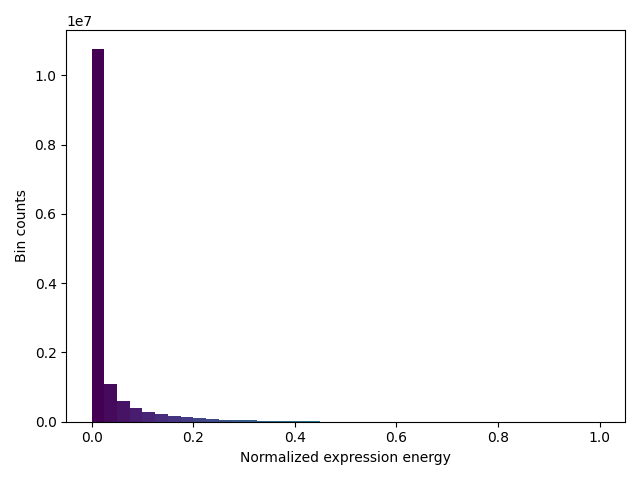
\includegraphics[width=.9\linewidth]{plotted_figures/global_normal_ge_data_histo.png}
		\caption{Histogram, globally norm}
		\label{fig:global_hist}
	\end{subfigure}
	\begin{subfigure}{.35\textwidth}
		\centering
		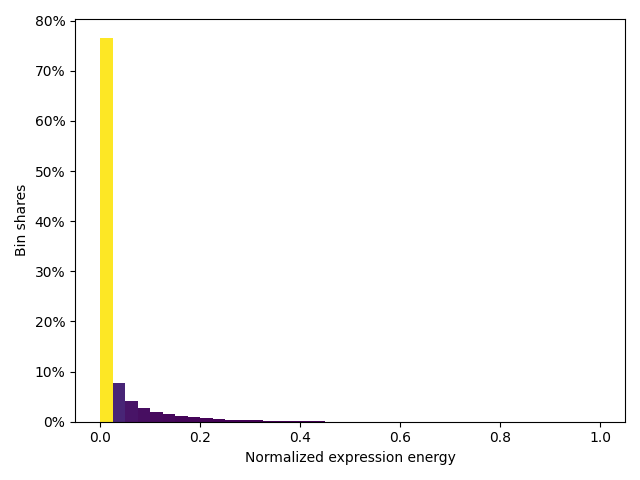
\includegraphics[width=.9\linewidth]{plotted_figures/global_percent_ge_data_histo.png}
		\caption{Bin shares, globally norm}
		\label{fig:global_perc}
	\end{subfigure}\\
	\begin{subfigure}{.35\textwidth}
		\centering
		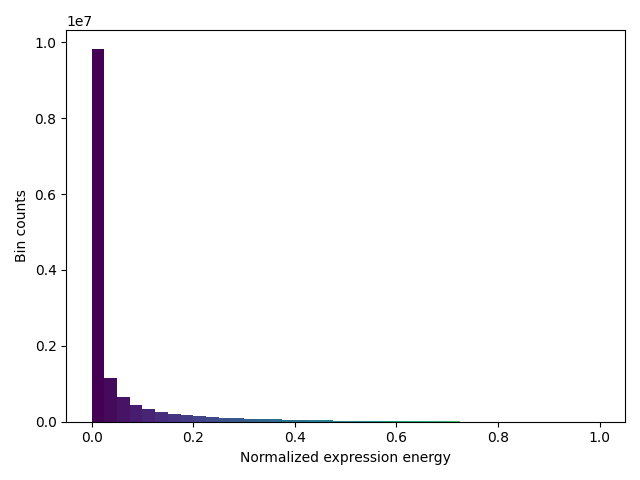
\includegraphics[width=.9\linewidth]{plotted_figures/row_normal_ge_data_histo.png}
		\caption{Histogram, row-wise norm}
		\label{fig:row_hist}
	\end{subfigure}
	\begin{subfigure}{.35\textwidth}
		\centering
		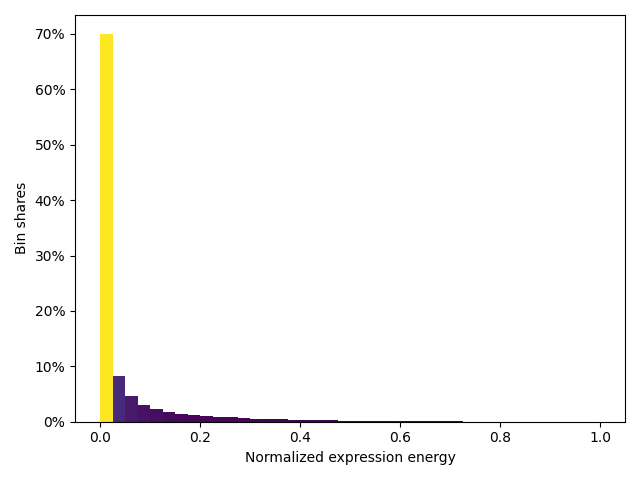
\includegraphics[width=.9\linewidth]{plotted_figures/row_percent_ge_data_histo.png}
		\caption{Bin shares, row-wise norm}
		\label{fig:row_perc}
	\end{subfigure}\\
	\begin{subfigure}{.35\textwidth}
		\centering
		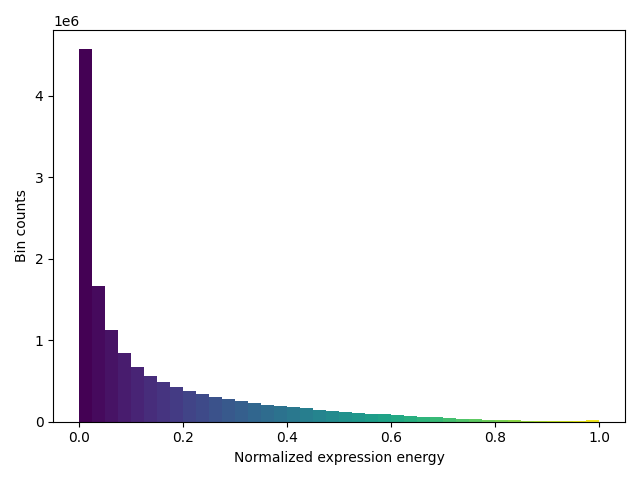
\includegraphics[width=.9\linewidth]{plotted_figures/column_normal_ge_data_histo.png}
		\caption{Histogram, column-wise norm}
		\label{fig:col_hist}
	\end{subfigure}
	\begin{subfigure}{.35\textwidth}
		\centering
		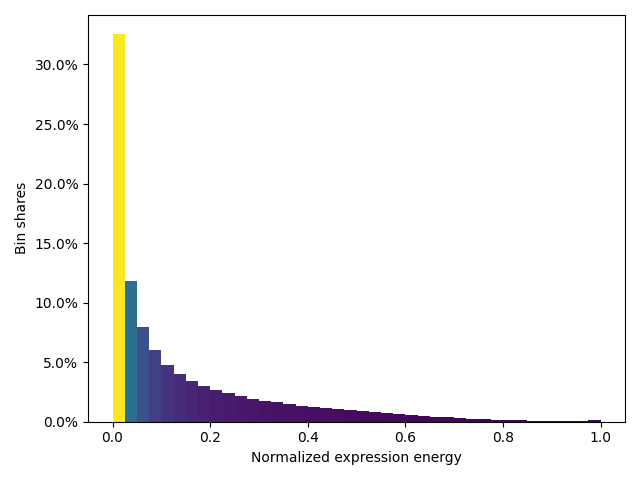
\includegraphics[width=.9\linewidth]{plotted_figures/column_percent_ge_data_histo.png}
		\caption{Bin shares, column-wise norm}
		\label{fig:col_perc}
	\end{subfigure}\\
	\caption{$|S|=843$, $|G|=16679$}
	\label{fig:ge_hists}
\end{figure}

\todo{Edit figure caption}

Especially for our binary classification task of gene expression prediction (see Section \ref{sec:probdesc_geneexp}), we need mapping of those entries to $\{0,1\}$. Moreover, neural networks prefer inputs in the interval $[0,1]$ as we want to use $M_{GE}$ as input for the problems described in Sections \ref{sec:probdesc_dimpres} and \ref{sec:probdesc_connpred}. Thus, we threshold the resulting normalized expression energies, by applying a fixed cut-off threshold $t\in[0,1]$. We experiment with various expression thresholds as described in results Section \ref{sec:results}.

\subsubsection{Protein-protein interaction graph}
As shortly sketched in the introduction (see Section \ref{sec:introduction}), we want to apply graph convolutional neural networks over protein-protein interaction (PPI) graphs and identify patterns within. However, there are numerous databases for PPI graphs publicly and freely available.
Common sources are CPDB\cite{lo2009cpdb}, iRefIndex\cite{razick2008irefindex}, MultiNet\cite{sengupta2023multinet} and STRING\cite{STRINGv10}. Due to our experience with the database and its success in other related tasks \cite{schulte2021integration, wang2021mogonet, hinnerichs2021dti}, we will use STRING (Version 10) as ground truth data. As STRING provide probabilities and hence confidence scores for each interaction, we re-use the recommended threshold of $0.7$ in order to retrieve only high-confidence interactions. STRING database contains $300000$ interactions between over $20000$ genes gathered from other databases and literature for \textit{Mus musculus}. An example interaction graph for \textit{Kdm7a}, an histone demethylase required for brain development, and its interactors is shown in Figure \ref{fig:PPI_graph}.

\begin{figure}
	\centering
	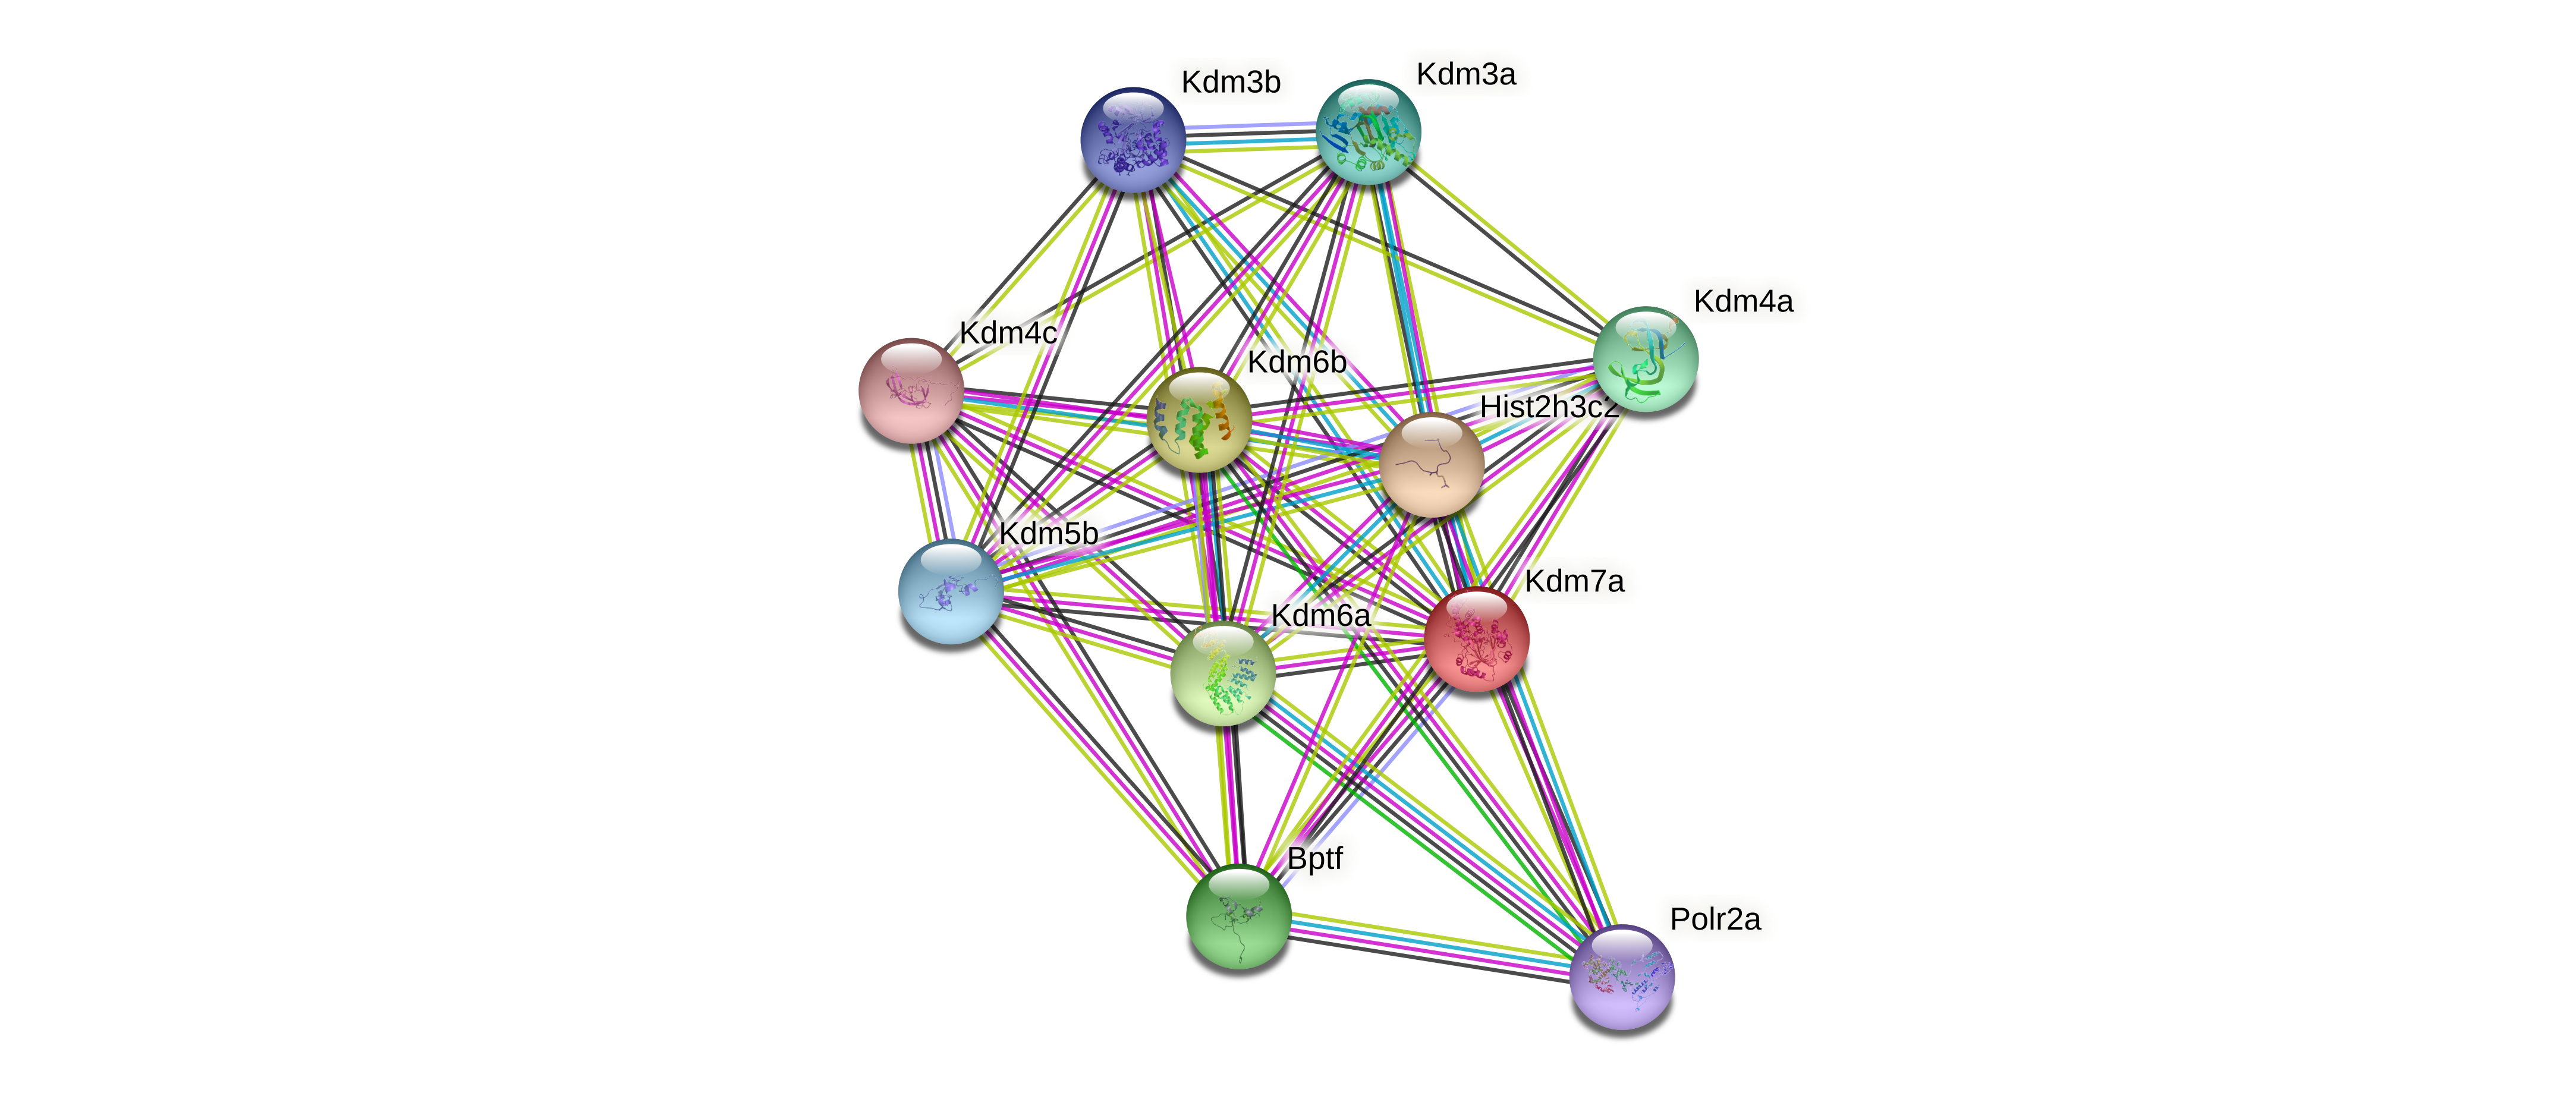
\includegraphics[width=1.\linewidth]{figures/string_hires_image.png}
	\caption{Protein-protein interaction graph for \textit{Kdm7a}, an histone demethylase required for brain development, that is closely related to e.g. \textit{Hist2h3c2}, a protein playing central role in transcription regulation and thus proliferation activity indicating e.g. malign tumors. For more information about \textit{Kdm7a} and the used color encoding for vertices and edges, please see \href{https://string-db.org/network/10090.ENSMUSP00000002305}{string-db.org/10090.ENSMUSP00000002305}}
	\label{fig:PPI_graph}
\end{figure}

\subsubsection{Structural connectome data}

We chose the AMBA partly with respect to its neat integration with the Allen Mouse Brain Connectivity Atlas (AMBCA)\cite{oh2014mesoscale}, published by the Allen institute, as a publicly available source for axonal connectivity data. The Allen Mouse Brain Connectivity Atlas is a high-resolution map of neuronal connections in the adult mouse brain, obtained from EGFP-expressing (enhanced green fluorescent protein) vectors following structural connections. As with AMBA, AMBCA tracing images were mapped back to 3D reference space using the CCF(v3) coordinates. Likewise, we are again able to group voxels to structures, parcelating the mouse brain and organized by the CCF ontology. All data was downloaded over the AllenSDK API. 

\subsubsection{Functional connectivity}
\begin{itemize}
	
	\item Where is data coming from? \cite{AIDAmri2019} (AIDAmri)
	\item How to calculate functional connectivity matrix $\rightarrow$ AIDAconnect (no paper yet? cite dataset?
	\item How to combine functional connectivity for multiple samples? 
\end{itemize}

\subsection*{in-depth description of the study design/datasets used and motivation why they were used for these experiments}
\subsection*{Explanation of Sample used in the study}

\begin{itemize}
	\item How did we achieve the matching?
	\item what are premises of the dataset?
	
	\item transfer learning working for other structure/regions
	\item dataset: Allen Mouse brain atlas vs. 
	\begin{itemize}
		\item \href{https://www.har.mrc.ac.uk/harwell-news/phenoview-new-tool-compare-impc-data/}{phenoview impc data}
		
		\item \href{https://www.mousephenotype.org/}{mousephenotype}
		
		\item \href{http://www.informatics.jax.org/expression.shtml}{HPO/MP project expression data}
	\end{itemize}
	\item Mouse brain CCFv3
\end{itemize}

Four graphs were used in this study:
\begin{itemize}
	\item Protein-protein interaction graph from STRING
	\item structure hierarchy/ontology from \cite{MouseBrainAtlas}
	\item structural connectivity data from (Mouse Projection data)
	\item functional connectivity data from \cite{AIDAmri2019}
	
\end{itemize}

\subsection{Model}
\label{sec:modeldesc}
\subsection*{Explanation of Measurement, Definitions, Indexes, Reliabililty and Validity of study method and study design}
\subsection*{Description of Analytical Tehcniques to be Applied and justification for them}

\subsection*{Reliability and validity of internal/external design and related subtypes}

\subsubsection{Feature generation}

Data preparation for regression task
\begin{itemize}
	\item unbalanced data for prediction task
\end{itemize}

\subsubsection{Graph convolutional neural layers}
\label{sec:graphconv}
We include these molecular and ontology-based sub-models within a
graph neural network (GNN) \cite{GCNConv}. The graph underlying the GNN is
based on the protein--protein interaction (PPI) graph. The PPI dataset
is represented by a graph $G=(V,E)$, where each protein is represented
by a vertex $v\in V$, and each edge $e\in E\subseteq V\times V$
represents an interaction between two proteins. Additionally, we
introduce a mapping $x:V\rightarrow\mathbb{R}^{d}$ projecting each
vertex $v$ to its node feature $x_v := x(v)$, where $d$ denotes the
dimensionality of the node features.

% As described before, graph convolution has shown significant
% performance increase in a variety of tasks. While there are various
% methods out there we will only introduce the most basic one here. 
A graph convolutional layer \cite{GCNConv} consists of a learnable
weight matrix followed by an aggregation step, formalized by
\begin{equation}
	\mathbf{X}^{\prime} = \mathbf{\hat{D}}^{-1/2} \mathbf{\hat{A}}
	\mathbf{\hat{D}}^{-1/2} \mathbf{X} \mathbf{\Theta}
\end{equation}
where for a given graph $G=(V,E)$, $\hat{A} = A + I$ denotes the
adjacency matrix with added self-loops for each vertex, $D$ is
described by $\hat{D}_{ii} = \sum_{j=0} \hat{A}_{ij}$, a diagonal
matrix displaying the degree of each node, and $\Theta$ denotes the
learnable weight matrix. Added self-loops enforce that each node
representation is directly dependent on its own preceding one. The
number of graph convolutional layers stacked equals the radius of
relevant nodes for each vertex within the graph.

The update rule for each node is given by a message passing scheme
formalized by
\begin{equation}
	\mathbf{x}^{\prime}_i = \mathbf{\Theta} \sum^{N}_{j}
	\frac{1}{\sqrt{\hat{d}_j \hat{d}_i}} \mathbf{x}_j
\end{equation}
where both $\hat{d}_i, \hat{d}_j$ are dependent on the edge weights
$e_{ij}$ of the graph. With simple, single-valued edge weights such as
$e_{ij}=1 \text{ }\forall (i,j)\in E$, all $\hat{d}_i$ reduce to
$d_i$, i.e., the degree of each vertex $i$. We denote this type of
graph convolutional neural layers with \textsc{GCNConv}.

While in this initial formulation of a GCNConv the node-wise update
step is defined by the sum over all neighboring node representations,
we can alter this formulation to other message passing schemes.  We
can rearrange the order of activation function $\sigma$, aggregation
$\mathrm{AGG}$, and linear neural layer $\mathrm{MLP}$ with this
formulation as proposed by \cite{GENConv2020}:
\begin{equation}
	\mathbf{x}_i^{\prime} = \mathrm{MLP} \left( \mathbf{x}_i +
	\mathrm{AGG} \left( \left\{
	\mathrm{\sigma} \left( \mathbf{x}_j + \mathbf{e_{ji}} \right) +\epsilon
	: j \in \mathcal{N}(i) \right\} \right)
	\right)
\end{equation}
where we only consider
$\sigma \in \{\mathrm{ReLU}, \mathrm{LeakyReLU}\}$. We denote this
generalized layer type as \textsc{GENConv} following the notation of
PyTorch Geometric \cite{PytorchGeometric}.  While the reordering is
mainly important for numerical stability, this alteration also addresses
the vanishing gradient problem for deeper convolutional networks
\cite{GENConv2020}. Additionally, we can also generalize the
aggregation function to allow different weighting functions such as
learnable $\mathrm{SoftMax}$ or $\mathrm{Power}$ for the incoming
signals for each vertex, substituting the averaging step in
\textsc{GCNConv}. Hence, while \textsc{GCNConv} suffers from both
vanishing gradients and signal fading for large scale and highly
connected graphs, each propagation step in \textsc{GENConv} emphasizes
signals with values close to $0$ and $1$. The same convolutional
filter and weight matrix are applied to and learned for all nodes
simultaneously. % , and the resulting information\todo{Which information?
% Specify} hold no information on their own connectivity.
We further employ another mechanism to avoid redundancy and fading
signals in stacked graph convolutional networks, using residual
connections and a normalization scheme \cite{DeepGCN2019}
	\cite{GENConv2020} as shown in Supplementary 3.  The residual
blocks are reusable and can be stacked multiple times.

\begin{itemize}
	\item what is GATConv?
	\item what is KerGNN and what is its idea?
	\item add some sentences to the section above
	\item node vs. graph classification vs. link prediction
\end{itemize}

\subsubsection{Dimensionality reduction techniques}
\paragraph{Principal component analysis (PCA)}
\label{sec:pca}

\paragraph{tSNE}
\label{sec:tsne}

\paragraph{UMAP}
\label{sec:umap}

\paragraph{Parametric UMAP}
\label{sec:paraumap}


\subsubsection{Hyperparameter tuning}
\begin{itemize}
	\item RayTune\cite{liaw2018tune} for automated hyperparameter tuning
\end{itemize}

\subsection{Evaluation and metrics}
\label{sec:evalmetrics}
\begin{itemize}
	\item AUC and AUPR for gene expression prediction
	\item self-built metric for evaluation of dim-red
	\item AUC and AUPR for conn pred
\end{itemize}


\newpage
\section{Results}
\label{sec:results}
\subsection{Gene expression prediction}


\begin{itemize}
	\item We originally started from the per section prediction in order to paste its performance and results to other "related" structures within in the mouse brain. We propose multiple ideas \dots. As mentioned we used three different feature types in this study. \dots (molecular features, phenotypical features, pure taxonomic features (InterPro embedding))) \dots Due to the poor performance of the predictor with all three used feature types, we abandoned these plane
	\item what is our baseline here? -> no study on prediction yet in adult mouse brains
	\begin{itemize}
		\item 
	\end{itemize}
	\item structure specific features?
	\begin{itemize}
		\item structural ontology / closeness
		\item developmental hierarchy of tissue
	\end{itemize}
\end{itemize}

Our model also allows us to test different ways of representing omics data. We
tested different ways to normalize values assigned to genes as these normalizations
convey different biological information; in the matrix of values assigned to genes from
cancer samples, we can normalize values across the entire matrix, across each row
(cancer sample), or across each column (gene). While a global normalization is more
common, row-based normalization allows us to highlight values that are significantly
higher or lower within one sample (e.g., which genes are expressed at high or low levels within a single sample), and column-based normalization allows us to highlight values
assigned to a particular gene that are significantly higher or lower within one sample
(e.g., whether a gene is expressed at higher or lower levels within one sample compared
to all others). We find that column-based normalization performs better than row-based
normalization, while the global normalization approach performs close to random. The
best results are achieved when combining both row- and column-based normalization
(Supplementary Table 2).	

\subsection{Dimensionality reduction and its combination with different graphs structures}

\begin{itemize}
	\item plot for showing validity of embeddings: K-means colour with respect to cluster 
	\item plot colour parent structure all similar
\end{itemize}

\subsection{On the linkage of connectivities and gene expression patterns}

\subsection*{Brief Overview of Material}
\subsection*{Findings (Results) of the Method of Study and Any Unplanned or Unexpected Situations that Occurred}
\subsection*{Brief Descriptive Analysis
Reliability and Validity of the Analysis}
\subsection*{Explanation of the Hypothesis and Precise and Exact Data (Do Not Give Your Opinion)}


\newpage
\section{Discussion}
\label{sec:discussion}
\subsection*{Brief Overview of Material}
\subsection*{Full Discussion of Findings (Results) and Implications}
\subsection*{Full Discussion of Research Analysis of Findings}
\subsection*{Full Discussion of Hypothesis and of Findings}
\subsection*{Post Analysis and Implications of Hypothesis and of Findings}

Novelty:
\begin{itemize}
	\item GCNs over gene expression was never applied here
\end{itemize}



\newpage
\section{Conclusion}
\label{sec:conclusion}

\subsection*{Summary of Academic Study}
\subsection*{Reference to Literature Review}
\subsection*{Implications of Academic Study}
\subsection*{Limitations of the Theory or Method of Research}
\subsection*{Recommendations or Suggestions of Future Academic Study}

\begin{itemize}
	\item gene expression patterns within mouse brain and both possible hypothesis and tasks, and models over this
	\item gene knockout models and whether they can learn propagation of those?
	\item connection of FC and gene expression patterns and how to prove such interaction/correlation?
	\item possible gene knockout targets within mouse brain and possible structural influences
\end{itemize}


\newpage

\bibliography{citations}

\end{document}